\documentclass[11pt,a4paper]{article}
\usepackage[margin=20mm]{geometry}
\usepackage{fontspec}
\setmainfont{Times New Roman}
\setmonofont{Courier New}
\usepackage[russian]{babel}
\usepackage{listings}
\usepackage{graphicx}
\usepackage[hidelinks]{hyperref}
\setlength{\parindent}{0pt}
\setlength{\parskip}{5pt}
\lstset{basicstyle=\ttfamily\fontsize{8.2}{9.5}\selectfont,
  columns=fullflexible,keepspaces=true,showstringspaces=false,
  breaklines=true,numbers=none,aboveskip=4pt,belowskip=6pt}
\newcommand{\head}[1]{\par\medskip{\large\bfseries #1}\par\nobreak\smallskip}
\newcommand{\subhead}[1]{\par\smallskip{\bfseries #1}\par\nobreak\smallskip}
\begin{document}
\thispagestyle{empty}
\begin{center}
{\bfseries МИНИСТЕРСТВО НАУКИ И ВЫСШЕГО ОБРАЗОВАНИЯ РОССИЙСКОЙ ФЕДЕРАЦИИ}\par
Федеральное государственное автономное образовательное учреждение высшего образования\par
{\bfseries «Московский авиационный институт (национальный исследовательский университет)»}\par
\vspace{30mm}
{\Large\bfseries ОТЧЁТ ПО ЛАБОРАТОРНОЙ РАБОТЕ}\par
{\Large\bfseries № 2}\par
\vspace{10mm}
{\bfseries Дисциплина:}\par
Операционные системы и архитектура компьютера\par
\vspace{6mm}
{\bfseries Тема:}\par
Процессы и неименованные каналы\par
Вариант 4
\end{center}
\vspace{20mm}
\begin{flushright}
{\bfseries Выполнил:}\par
студент группы М8О-202БВ-25\par
Григорьев Глеб Алексеевич\par
\vspace{7mm}
{\bfseries Проверил:}\par
Ассистент Центра ТОП-ИТ\par
Ефимов Д.А.
\end{flushright}
\vfill
\begin{center}Москва, 2026 г.\end{center}
\newpage
\head{1. Цель работы}
Разработать две программы на Си, которые обмениваются данными через неименованные каналы. Реализовать последовательное деление чисел типа float в дочернем процессе, запись результатов в файл и завершение обоих процессов при нулевом делителе.

\head{2. Краткое описание архитектуры решения}
Родительская программа parent получает имя выходного файла и строки с числами. Программа child выполняет вычисления и записывает результаты. Общие функции обмена вынесены в ipc.c, объявления и коды состояний — в ipc.h. Проект собирается через Makefile.

Два канала создаются до fork. Через pipe1 родитель передаёт строки в стандартный ввод дочернего процесса. Через pipe2 возвращаются ответы: R — файл открыт, K — результат записан, Z — нулевой делитель, E — ошибка. Имя файла передаётся аргументом execl. После каждой команды родитель ждёт ответ.

Для строк используются динамические буферы getline. SIGPIPE игнорируется, чтобы обрыв канала обрабатывался как ошибка записи. Перед завершением освобождаются буферы и закрываются дескрипторы; родитель вызывает waitpid.

\subhead{2.1 Схема взаимодействия компонентов}
\begin{center}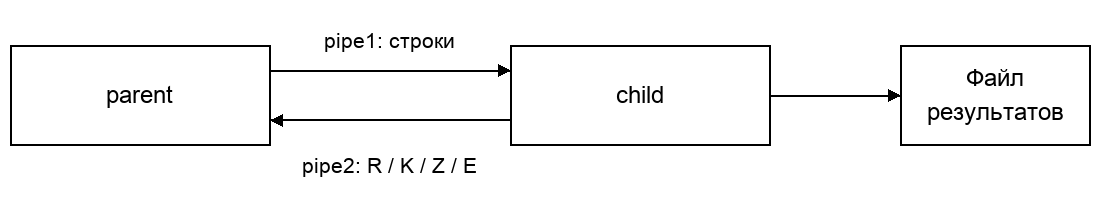
\includegraphics[width=0.931\linewidth]{assets/ipc-schema.png}\end{center}
\begin{center}\small Рисунок 1 — Архитектура решения\end{center}
\head{3. Листинг ключевых фрагментов кода}
Полные исходники: \url{https://github.com/Geegunt/LabsOSI/tree/main/Lab2/src}
\subhead{3.1 Создание каналов и запуск дочернего процесса}
Родитель создаёт каналы и дочерний процесс. В дочерней ветке stdin и stdout перенаправляются на каналы, затем запускается отдельная программа child.

\lstinputlisting[firstline=45,lastline=70]{../src/parent.c}
\begin{center}\small Листинг 1 — Инициализация IPC и запуск child в parent.c\end{center}
\newpage
\subhead{3.2 Преобразование чисел и деление}
Первое число сохраняется в result. Каждый следующий делитель проверяется на ноль до выполнения операции. strtof позволяет проверить, что число прочитано полностью и находится в допустимом диапазоне.

\lstinputlisting[firstline=21,lastline=41]{../src/child.c}
\begin{center}\small Листинг 2 — Разбор чисел и проверка делителя в child.c\end{center}
\subhead{3.3 Передача данных через канал}
write может передать только часть строки. Функция повторяет запись оставшихся байтов, а при EINTR повторяет прерванный вызов.

\lstinputlisting[firstline=7,lastline=23]{../src/ipc.c}
\begin{center}\small Листинг 3 — Запись строки целиком в ipc.c\end{center}
SIGPIPE игнорируется, поэтому обрыв канала обрабатывается как ошибка write. При закрытии канала ответов родитель получает EOF. Ошибки системных вызовов проверяются, сообщения выводятся в stderr.

Перед завершением освобождаются буферы getline, закрываются файл и дескрипторы каналов. Родитель вызывает waitpid. При обычном конце ввода запись в pipe1 закрывается, дочерний процесс получает EOF и завершает работу.

\newpage
\head{4. Результаты работы}
Проверка выполнена 18 ноября 2026 года в контейнере Debian 12, Linux aarch64. Использовались GCC 12.2, Python 3.11 и strace 6.1. Команды сборки и тестирования:

\begin{lstlisting}
make clean
make
make test
\end{lstlisting}
Сборка с -Wall -Wextra -Wpedantic -Werror завершилась без предупреждений. Прошли все 18 тестов, включая запись в /dev/full, длинные строки, ошибочный ввод и завершение по нулевому делителю.

\subhead{4.1 Консольный вывод или логи}
Для строк «100 2 5», «7.5 2.5» и «0 2» в файле получены 10, 3 и 0. Ниже приведены строки журнала normal.log с PID процессов:

\begin{lstlisting}
[parent PID=890] Output file: [parent PID=890] child PID=891
[child PID=891 PPID=890] Started
[parent PID=890] Numbers (Ctrl+D to finish): [child PID=891] Result: 10
[parent PID=890] Numbers (Ctrl+D to finish): [child PID=891] Result: 3
[parent PID=890] Numbers (Ctrl+D to finish): [child PID=891] Result: 0
[parent PID=890] Numbers (Ctrl+D to finish): [parent PID=890] Child exit code: 0
\end{lstlisting}
\subhead{Проверка нулевого делителя}
На вход поданы «20 2», «10 0» и «99 3». В файле остался только результат 10. Третья команда не выполнена, оба процесса завершились с кодом 2. Фрагмент zero.log:

\begin{lstlisting}
[parent PID=897] Output file: [parent PID=897] child PID=898
[child PID=898 PPID=897] Started
[parent PID=897] Numbers (Ctrl+D to finish): [parent PID=897] Division by zero; stopping
[parent PID=897] Child exit code: 2
\end{lstlisting}
В журналах видны PID родительских и дочерних процессов: 890/891 и 897/898. Запись результатов подтверждается сообщениями Result и содержимым файлов. Завершение процессов дополнительно проверено по exit\_group и wait4 в трассировке.

\subhead{4.2 Скриншоты результатов}
На рисунке приведены фрагменты сохранённой трассировки normal.strace. Видны создание каналов, запуск child, запись результата и получение статуса дочернего процесса. Полные журналы находятся в report/assets/linux.

\begin{center}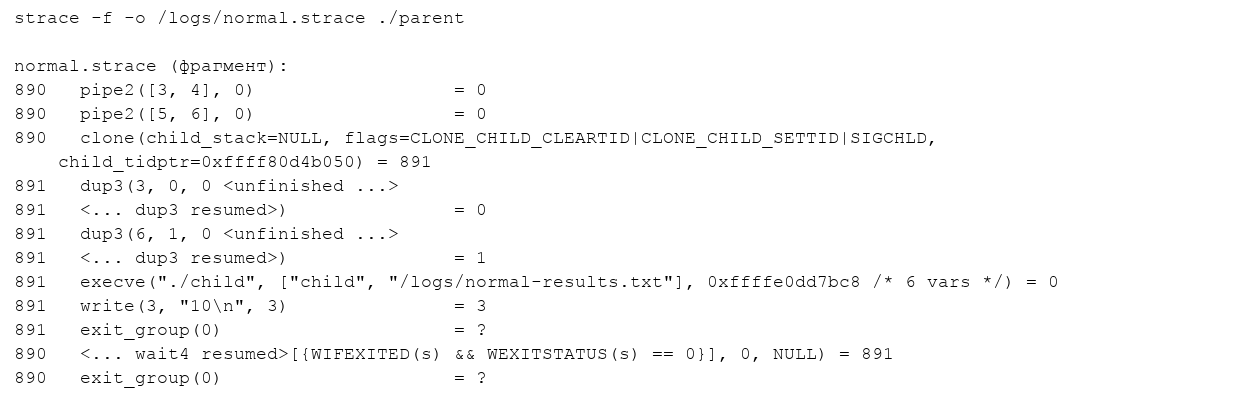
\includegraphics[width=0.993\linewidth]{assets/linux-trace.png}\end{center}
\begin{center}\small Рисунок 2 — Фрагменты трассировки обычного запуска в Linux\end{center}
В этой Linux-среде вызовы fork, dup2 и waitpid отображаются как clone, dup3 и wait4.

\head{5. Выводы}
Реализован обмен между родительским и дочерним процессами через два неименованных канала. Дочерняя программа выполняет деление и записывает результаты в файл; при нулевом делителе оба процесса завершаются. Работа подтверждена 18 Linux-тестами, журналами с PID и трассировкой strace; отработаны создание процесса, перенаправление потоков и освобождение ресурсов.

\end{document}
